
\noindent \textbf{L2.2 (Sipser 1.6c)} Dê um DFA/AFD para $A = \{w | w$ possui $0101$ por subcadeia\}.

\begin{figure}[!h]
\centering
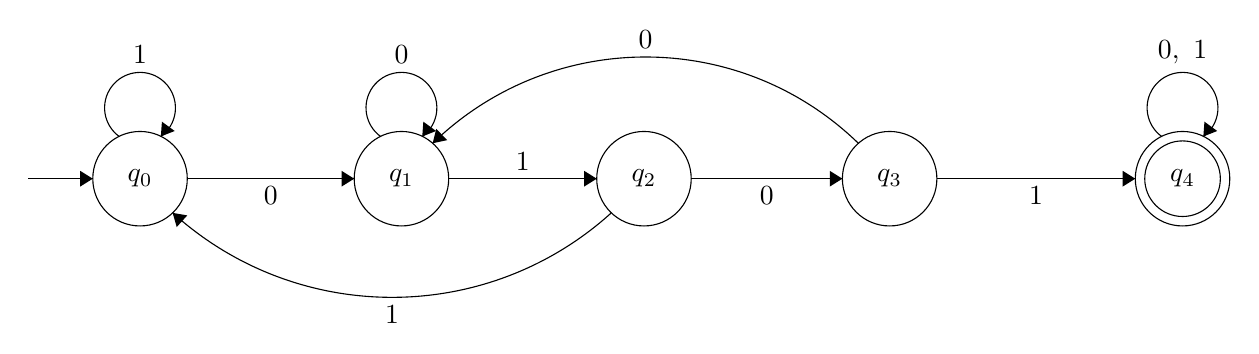
\begin{tikzpicture}[scale=0.2]
    \tikzstyle{every node}+=[inner sep=0pt]
    \draw [black] (7.9,-19.1) circle (3);
    \draw (7.9,-19.1) node {$q_0$};
    \draw [black] (24.5,-19.1) circle (3);
    \draw (24.5,-19.1) node {$q_1$};
    \draw [black] (39.9,-19.1) circle (3);
    \draw (39.9,-19.1) node {$q_2$};
    \draw [black] (55.5,-19.1) circle (3);
    \draw (55.5,-19.1) node {$q_3$};
    \draw [black] (74.1,-19.1) circle (3);
    \draw (74.1,-19.1) node {$q_4$};
    \draw [black] (74.1,-19.1) circle (2.4);
    \draw [black] (0.8,-19.1) -- (4.9,-19.1);
    \fill [black] (4.9,-19.1) -- (4.1,-18.6) -- (4.1,-19.6);
    \draw [black] (10.9,-19.1) -- (21.5,-19.1);
    \fill [black] (21.5,-19.1) -- (20.7,-18.6) -- (20.7,-19.6);
    \draw (16.2,-19.6) node [below] {$0$};
    \draw [black] (27.5,-19.1) -- (36.9,-19.1);
    \fill [black] (36.9,-19.1) -- (36.1,-18.6) -- (36.1,-19.6);
    \draw (32.2,-18.6) node [above] {$1$};
    \draw [black] (42.9,-19.1) -- (52.5,-19.1);
    \fill [black] (52.5,-19.1) -- (51.7,-18.6) -- (51.7,-19.6);
    \draw (47.7,-19.6) node [below] {$0$};
    \draw [black] (58.5,-19.1) -- (71.1,-19.1);
    \fill [black] (71.1,-19.1) -- (70.3,-18.6) -- (70.3,-19.6);
    \draw (64.8,-19.6) node [below] {$1$};
    \draw [black] (6.577,-16.42) arc (234:-54:2.25);
    \draw (7.9,-11.85) node [above] {$1$};
    \fill [black] (9.22,-16.42) -- (10.1,-16.07) -- (9.29,-15.48);
    \draw [black] (23.177,-16.42) arc (234:-54:2.25);
    \draw (24.5,-11.85) node [above] {$0$};
    \fill [black] (25.82,-16.42) -- (26.7,-16.07) -- (25.89,-15.48);
    \draw [black] (26.483,-16.853) arc (134.14834:45.85166:19.407);
    \fill [black] (26.48,-16.85) -- (27.41,-16.65) -- (26.71,-15.94);
    \draw (40,-10.87) node [above] {$0$};
    \draw [black] (37.829,-21.267) arc (-47.84822:-132.15178:20.755);
    \fill [black] (9.97,-21.27) -- (10.23,-22.17) -- (10.9,-21.43);
    \draw (23.9,-27.13) node [below] {$1$};
    \draw [black] (72.777,-16.42) arc (234:-54:2.25);
    \draw (74.1,-11.85) node [above] {$0,\mbox{ }1$};
    \fill [black] (75.42,-16.42) -- (76.3,-16.07) -- (75.49,-15.48);
\end{tikzpicture}
\caption{Diagrama de estados do AFD que reconhece $A$.}
\label{fig:sip1.6c}
\end{figure}
